\section{Modular Curves}\label{Sec:MF_modular_curves}
\subsection{Riemann Surfaces}\label{Sec:MF_Riemann_surfaces}
\begin{definition}
    A \termino{complete one-dimensional complex atlas} on a Hausdorff topological space $X$ is a collection $\{(U_i, \varphi_i)\}_{i \in I}$ satisfying:
    \begin{enumerate}[label=(\arabic*)]
        \item $\{U_i\}_{i \in I}$ is an open cover of $X$.
        \item Each $\varphi_i : U_i \to \bbC$ is a homeomorphism onto its image.
        % The notes do not explicitly require the chart images to be open in C; this was reported and remains pending confirmation.
        \item For every $i, j \in I$, the transition map
        \[
            \varphi_j \circ \varphi_i^{-1} : \varphi_i(U_i \cap U_j) \to \varphi_j(U_i \cap U_j)
        \]
        is holomorphic.
        \item If $V \subseteq X$ is open and $\psi : V \to \bbC$ is a homeomorphism onto its image such that $\psi \circ \varphi_i^{-1}$ is holomorphic on $\varphi_i(U_i \cap V)$ for every $i \in I$, then $(V, \psi)$ belongs to the atlas.
    \end{enumerate}
\end{definition}

\begin{definition}
    A \termino{Riemann surface} is a connected Hausdorff topological space equipped with a complete one-dimensional complex atlas. It is \termino{compact} if its underlying topological space is compact.
\end{definition}

\begin{example}
    \leavevmode
    \begin{enumerate}[label=(\arabic*)]
        \item Noncompact examples include $\bbC$, connected subsets of $\bbC$ and modular curves $Y(\Gamma)$.
        % The notes say "connected subsets"; the missing openness condition was reported and remains pending confirmation.
        \item Compact examples include the Riemann sphere $\widehat{\bbC} = \bbC \cup \{\infty\}$, complex tori $\bbC/\Lambda$, modular curves $X(\Gamma)$ and $g$-holed tori.
    \end{enumerate}
\end{example}

\begin{definition}\label{Def:MF_holomorphic_map}
    A map $f : X \to Y$ between Riemann surfaces is \termino{holomorphic} if it is continuous and, for every chart $(U, \varphi)$ on $X$ and $(V, \psi)$ on $Y$ with $f(U) \subseteq Y$, the coordinate expression
    \[
        \psi \circ f \circ \varphi^{-1} : \varphi(U) \to \psi(V)
    \]
    is holomorphic.
    % The notes write f(U) subset Y; replacing Y by V was proposed and remains pending confirmation.
\end{definition}

\begin{proposition}[Local Normal Form]\label{Prop:MF_local_normal_form}
    Let $f : X \to Y$ be a nonconstant holomorphic map between Riemann surfaces, $x \in X$ and $y = f(x)$. There exist an integer $e_x > 0$ and charts $(U, \varphi)$ on $X$ and $(V, \psi)$ on $Y$ such that:
    \begin{enumerate}[label=(\arabic*)]
        \item $x \in U$, $\varphi(x) = 0$, $y \in V$ and $\psi(y) = 0$.
        \item $f(U) \subseteq V$.
        \item In these coordinates,
        \[
            \psi \circ f \circ \varphi^{-1} : \varphi(U) \to \psi(V), \quad z \mapsto z^{e_x}.
        \]
    \end{enumerate}
\end{proposition}

\begin{proof}[Sketch of proof]
    Choose charts satisfying (1) and (2), and put $h = \psi \circ f \circ \varphi^{-1}$. By the identity theorem, $h$ is nonconstant. Since $h(0) = 0$, write
    \[
        h(z) = z^m g(z), \quad m > 0, \quad g(0) \neq 0,
    \]
    where $g$ is holomorphic. After shrinking the charts, choose a holomorphic $m$-th root of $g$. The map
    \[
        t(z) = z\sqrt[m]{g(z)}
    \]
    fixes $0$ and has nonzero derivative $t'(0) = \sqrt[m]{g(0)}$. Shrinking the charts again, $t$ is biholomorphic. Replacing $\varphi$ by $t \circ \varphi$, the coordinate expression of $f$ becomes $z \mapsto z^m$.
\end{proof}

\begin{definition}\label{Def:MF_ramification}
    Let $f : X \to Y$ be a nonconstant holomorphic map. The integer $e_x$ in \propref{Prop:MF_local_normal_form} is the \termino{ramification index} at $x$. A point $x$ is a \termino{ramification point} if $e_x > 1$. Write
    \[
        R(f) \defeq \{x \in X \mid e_x > 1\}.
    \]
\end{definition}

\begin{corollary}\label{Cor:MF_discrete_fibres}
    Let $f : X \to Y$ be a nonconstant holomorphic map between Riemann surfaces.
    \begin{enumerate}[label=(\arabic*)]
        \item For every $y \in Y$, the fibre $f^{-1}(y)$ is a closed discrete subset of $X$.
        \item $R(f)$ is a closed discrete subset of $X$.
    \end{enumerate}
    In particular, if $X$ is compact, then $f^{-1}(y)$ and $R(f)$ are finite.
\end{corollary}

\begin{proof}
    Locally, $f$ has the form $z \mapsto z^m$, which has discrete fibres and at most one ramification point, namely $0$ when $m > 1$. The fibre is closed by continuity, and the local normal form also shows that the complement of $R(f)$ is open. Closed discrete subsets of a compact space are finite.
\end{proof}

\begin{corollary}\label{Cor:MF_open_map}
    A nonconstant holomorphic map between Riemann surfaces is open.
\end{corollary}

\begin{proof}
    Locally, the map has the form $z \mapsto z^m$, which is open.
\end{proof}

\begin{corollary}\label{Cor:MF_compact_surjective}
    Let $f : X \to Y$ be a holomorphic map between Riemann surfaces. If $X$ is compact, then $f$ is either constant or surjective.
\end{corollary}

\begin{proof}
    Assume $f$ is nonconstant.
    \begin{itemize}
        \item $f(X)$ is open in $Y$ by \corref{Cor:MF_open_map}.
        \item $f(X)$ is compact. Since $Y$ is Hausdorff, $f(X)$ is closed in $Y$.
    \end{itemize}
    Since $Y$ is connected, $f(X) = Y$.
\end{proof}

\begin{thmdef}[Degree]\label{Def:MF_degree}
    Let $f : X \to Y$ be a holomorphic map between Riemann surfaces with $X$ compact. The \termino{degree} of $f$ is the integer
    \[
        \deg(f) \defeq \sum_{x \in f^{-1}(y)}e_x,
    \]
    independent of the choice of $y \in Y$.
    % The board omits the nonconstant hypothesis; this was reported and remains pending confirmation.
\end{thmdef}

\begin{proof}[Sketch of proof]
    One needs to check independence of $y$. Away from the branch values, use the covering map supplied by the local normal form. An evenly covered neighbourhood has inverse image a disjoint union of open sets, each mapped homeomorphically onto that neighbourhood. Near a ramification point, the local expression $z \mapsto z^{e_x}$ accounts for the multiplicity $e_x$.
    % The board writes X minus R(f) -> Y minus f(R(f)). The proposed source is X minus f^{-1}(f(R(f))); this correction remains pending confirmation. The bottom of the photographed proof is cut off.
\end{proof}

\subsection{Complex Tori}\label{Sec:MF_complex_tori}
\begin{definition}\label{Def:MF_lattice}
    A \termino{lattice} in $\bbC$ is a subgroup
    \[
        \Lambda = \bbZ\omega_1 \oplus \bbZ\omega_2 \subseteq \bbC,
    \]
    where $\{\omega_1, \omega_2\}$ is a basis of $\bbC$ over $\bbR$.
\end{definition}

We adopt the convention that $\omega_1/\omega_2 \in \calH$.

\begin{lemma}\label{Lem:MF_lattice_basis}
    Let $\Lambda = \bbZ\omega_1 \oplus \bbZ\omega_2$ and $\Lambda' = \bbZ\omega'_1 \oplus \bbZ\omega'_2$ be lattices with bases satisfying the above convention. Then $\Lambda = \Lambda'$ if and only if there exists $g \in \SL_2(\bbZ)$ such that
    \[
        \begin{pmatrix}\omega'_1\\ \omega'_2\end{pmatrix} = g\begin{pmatrix}\omega_1\\ \omega_2\end{pmatrix}.
    \]
\end{lemma}

\begin{proof}
    \leavevmode
    \begin{enumerate}[label=(\arabic*)]
        \item Suppose $\Lambda = \Lambda'$. There exists $g = \begin{pmatrix}a & b\\ c & d\end{pmatrix} \in \GL_2(\bbZ)$ taking one basis to the other. Put $z = \omega_1/\omega_2$ and $z' = \omega'_1/\omega'_2$. Then
        \[
            gz = \frac{az + b}{cz + c} = \frac{a\omega_1 + b\omega_2}{c\omega_1 + d\omega_2} = \frac{\omega'_1}{\omega'_2} = z'.
        \]
        % The first denominator cz+c is transcribed from the handwritten notes; changing it to cz+d was proposed and remains pending confirmation.
        Since $z, z' \in \calH$, \propref{Prop:MF_imaginary_part} implies $\det(g) > 0$. As $\det(g) = \pm 1$, we have $\det(g) = 1$.
        \item Conversely, a matrix in $\SL_2(\bbZ)$ is an invertible integral change of basis, so the two bases generate the same lattice.
    \end{enumerate}
\end{proof}

\begin{definition}\label{Def:MF_complex_torus}
    A \termino{complex torus} is a quotient of $\bbC$ by a lattice $\Lambda$:
    \[
        \bbC/\Lambda = \{z + \Lambda \mid z \in \bbC\}.
    \]
\end{definition}

\begin{remark}
    \leavevmode
    \begin{itemize}
        \item A complex torus is an abelian group, as a quotient of $(\bbC, +)$ by $\Lambda$.
        \item A complex torus is a compact Riemann surface.
    \end{itemize}
    In particular, a holomorphic map $\bbC/\Lambda \to \bbC/\Lambda'$ is either constant or surjective by \corref{Cor:MF_compact_surjective}.
\end{remark}

\begin{proposition}\label{Prop:MF_torus_maps}
    Let $f : \bbC/\Lambda \to \bbC/\Lambda'$ be holomorphic. There exist $m, b \in \bbC$ such that:
    \begin{enumerate}[label=(\arabic*)]
        \item $m\Lambda \subseteq \Lambda'$.
        \item $f(z + \Lambda) = mz + b + \Lambda'$.
    \end{enumerate}
    Moreover, $f$ is invertible if and only if $m\Lambda = \Lambda'$.
\end{proposition}

\begin{proof}
    \leavevmode
    \begin{enumerate}[label=\textit{Step~\arabic*.}]
        \item Since $\bbC$ is a universal cover of $\bbC/\Lambda'$, the composite $\bbC \to \bbC/\Lambda \xrightarrow{f} \bbC/\Lambda'$ admits a lift $\widetilde f : \bbC \to \bbC$. The covering-space justification is deferred to a later reference. The lift is holomorphic because $f$ is holomorphic.

        \item Fix $\lambda \in \Lambda$ and define
        \[
            g_\lambda(z) \defeq \widetilde f(z + \lambda) - \widetilde f(z).
        \]
        Since $\widetilde f$ is a lift, $g_\lambda$ takes values in $\Lambda'$. It is continuous, $\bbC$ is connected and $\Lambda'$ is discrete, so $g_\lambda$ is constant. Differentiating gives
        \[
            \widetilde f'(z + \lambda) = \widetilde f'(z).
        \]
        Thus $\widetilde f'$ is entire and $\Lambda$-periodic, hence bounded on $\bbC$. By Liouville's theorem it is constant. Therefore
        \[
            \widetilde f(z) = mz + b.
        \]
        The lifting property gives $m\Lambda \subseteq \Lambda'$ and $f(z + \Lambda) = mz + b + \Lambda'$.

        \item For the invertibility assertion, the board argues that if $m\Lambda \neq \Lambda'$, one can choose $z \in \Lambda'$ with $z/m \notin \Lambda$. Then
        \[
            f(z/m + \Lambda) = b + \Lambda' = f(0 + \Lambda),
        \]
        so $f$ is not injective. If $m\Lambda = \Lambda'$, the inverse is induced by an affine map on $\bbC$.
        % The m=0 case is not treated on the board before division by m; this gap was reported. The photographed inverse has +b/m, whereas the proposed correction is -b/m. Both points remain pending confirmation; the explicit inverse formula is left out here.
    \end{enumerate}
\end{proof}

\begin{proposition}\label{Prop:MF_torus_homomorphism}
    Let $f : \bbC/\Lambda \to \bbC/\Lambda'$ be the holomorphic map $f(z + \Lambda) = mz + b + \Lambda'$ with $m\Lambda \subseteq \Lambda'$. The following are equivalent:
    \begin{enumerate}[label=(\arabic*)]
        \item $f$ is a group homomorphism.
        \item $b \in \Lambda'$, so $f(z + \Lambda) = mz + \Lambda'$.
        \item $f(0) = 0$.
    \end{enumerate}
\end{proposition}

\begin{proof}
    \leavevmode
    \begin{enumerate}[label=(\arabic*)]
        \item (1) $\implies$ (3) is immediate.
        \item (3) $\implies$ (2): $f(0 + \Lambda) = b + \Lambda'$, so $f(0) = 0$ if and only if $b \in \Lambda'$.
        \item (2) $\implies$ (1): the map is $z + \Lambda \mapsto mz + \Lambda'$, which is a group homomorphism.
    \end{enumerate}
\end{proof}

\begin{corollary}\label{Cor:MF_torus_isogeny}
    \leavevmode
    \begin{enumerate}[label=(\arabic*)]
        \item There exists a nonzero holomorphic group homomorphism $\bbC/\Lambda \to \bbC/\Lambda'$ if and only if there exists $m \in \bbC^\times$ such that $m\Lambda \subseteq \Lambda'$.
        \item There exists a holomorphic group isomorphism $\bbC/\Lambda \to \bbC/\Lambda'$ if and only if there exists $m \in \bbC^\times$ such that $m\Lambda = \Lambda'$.
    \end{enumerate}
\end{corollary}

\begin{proof}
    Apply \propref{Prop:MF_torus_maps} and \propref{Prop:MF_torus_homomorphism}.
\end{proof}

\begin{definition}\label{Def:MF_isogeny}
    A nonzero holomorphic group homomorphism between complex tori is an \termino{isogeny}.
\end{definition}

\begin{remark}
    If $f : \bbC/\Lambda \to \bbC/\Lambda'$ is the isogeny $f(z + \Lambda) = mz + \Lambda'$, then
    \[
        \ker(f) = m^{-1}\Lambda'/\Lambda = f^{-1}(\{0\})
    \]
    is finite by \corref{Cor:MF_discrete_fibres}.
\end{remark}

\begin{example}[Multiplication by an Integer]\label{Ex:MF_multiplication}
    Let $m \in \bbN_{>0}$ and let $\Lambda$ be a lattice. Define
    \[
        [m] : \bbC/\Lambda \to \bbC/\Lambda, \quad z + \Lambda \mapsto mz + \Lambda.
    \]
    Since $m\Lambda \subseteq \Lambda$, this is an isogeny. Moreover,
    \[
        \ker([m]) = m^{-1}\Lambda/\Lambda \cong (\bbZ/m\bbZ)^2.
    \]
    If $E = \bbC/\Lambda$, we write
    \[
        E[m] \defeq \ker([m] : E \to E)
    \]
    for its \termino{$m$-torsion subgroup}.
\end{example}

\begin{example}[Quotient by a Cyclic Subgroup]\label{Ex:MF_cyclic_quotient}
    Let $E = \bbC/\Lambda$, $m \in \bbN_{>0}$ and let $C \subseteq E[m]$ be a cyclic subgroup. Under the quotient map $\bbC \to E$, the subgroup $C$ corresponds to a lattice $\Lambda_C \supseteq \Lambda$, namely
    \[
        \Lambda_C = \{z \in \bbC \mid z + \Lambda \in C\}.
    \]
    Define
    \[
        \pi_C : \bbC/\Lambda \to \bbC/\Lambda_C, \quad z + \Lambda \mapsto z + \Lambda_C.
    \]
    Then $\pi_C$ is an isogeny with $\ker(\pi_C) = C$.
\end{example}

\begin{proposition}\label{Prop:MF_isogeny_factorization}
    Let $f : E = \bbC/\Lambda \to \bbC/\Lambda'$ be an isogeny given by $f(z + \Lambda) = mz + \Lambda'$, and put $K = \ker(f)$. Then $f$ is a composite of multiplication by a positive integer, a quotient by a cyclic subgroup and an isomorphism.
\end{proposition}

\begin{proof}
    \leavevmode
    \begin{enumerate}[label=\textit{Step~\arabic*.}]
        \item Put $N = |K|$. Then $K \subseteq E[N] \cong (\bbZ/N\bbZ)^2$, so there exist $n, n' \in \bbN_{>0}$ such that
        \[
            K \cong \bbZ/n\bbZ \times \bbZ/(nn')\bbZ.
        \]
        Multiplication by $n$ maps $K$ onto the cyclic subgroup $nK \cong \bbZ/n'\bbZ$.

        \item Write $\widetilde K = m^{-1}\Lambda'$ for the lattice corresponding to $K$, so $K = \widetilde K/\Lambda$. The lattice corresponding to $nK$ is $n\widetilde K$. Consider the quotient isogeny
        \[
            \pi : \bbC/\Lambda \to \bbC/(n\widetilde K), \quad z + \Lambda \mapsto z + n\widetilde K,
        \]
        whose kernel is $nK$.

        \item The map
        \[
            \iota : \bbC/(n\widetilde K) \to \bbC/\Lambda', \quad z + n\widetilde K \mapsto \frac{m}{n}z + \Lambda'
        \]
        is an isomorphism, since
        \[
            \frac{m}{n}(n\widetilde K) = m\widetilde K = \Lambda'.
        \]
        By construction,
        \[
            \begin{tikzcd}
                \bbC/\Lambda \arrow[r, "{[n]}"] & \bbC/\Lambda \arrow[r, "\pi"] & \bbC/(n\widetilde K) \arrow[r, "\iota", "\sim"'] & \bbC/\Lambda'
            \end{tikzcd}
        \]
        sends $z + \Lambda$ to $nz + \Lambda$, then to $nz + n\widetilde K$, and finally to $mz + \Lambda'$. Thus $f = \iota \circ \pi \circ [n]$.
    \end{enumerate}
\end{proof}

\begin{thmdef}[Dual Isogeny]\label{Def:MF_dual_isogeny}
    Let $f : \bbC/\Lambda \to \bbC/\Lambda'$ be an isogeny given by $f(z + \Lambda) = mz + \Lambda'$. Choose a basis $\{\omega'_1, \omega'_2\}$ of $\Lambda'$ and positive integers $m_1, m_2$ such that $\{m_1\omega'_1, m_2\omega'_2\}$ is a basis of $m\Lambda$. The \termino{dual isogeny} of $f$ is
    \[
        \widehat f : \bbC/\Lambda' \to \bbC/\Lambda, \quad z + \Lambda' \mapsto \frac{m_1m_2}{m}z + \Lambda.
    \]
    Moreover,
    \[
        \deg(f) = m_1m_2, \qquad \widehat f \circ f = [\deg(f)].
    \]
\end{thmdef}

\begin{proof}
    Since $m\Lambda \subseteq \Lambda'$, such bases and integers may be chosen. We have
    \[
        m_1m_2\Lambda' \subseteq m\Lambda, \qquad \frac{m_1m_2}{m}\Lambda' \subseteq \Lambda,
    \]
    so the displayed formula defines an isogeny. Its composite with $f$ satisfies
    \[
        (\widehat f \circ f)(z + \Lambda) = \frac{m_1m_2}{m}mz + \Lambda = m_1m_2z + \Lambda.
    \]
    The map $f$ has nonzero derivative in local coordinates, so each ramification index is $1$. Its fibres are translates of its kernel, and
    \[
        |\ker(f)| = [\Lambda' : m\Lambda] = m_1m_2.
    \]
    Hence $\deg(f) = m_1m_2$ and $\widehat f \circ f = [\deg(f)]$.
\end{proof}

\begin{remarkstar}
    Further properties of dual isogenies are left as exercises.
\end{remarkstar}

\begin{definition}[Weil Pairing]\label{Def:MF_Weil_pairing}
    Let $E = \bbC/\Lambda$ and $N \in \bbN_{>0}$. Choose a basis $\{\omega_1, \omega_2\}$ of $\Lambda$ with $\omega_1/\omega_2 \in \calH$. Then
    \[
        E[N] \cong (\bbZ/N\bbZ)^2 = \left\langle\frac{\omega_1}{N} + \Lambda\right\rangle \times \left\langle\frac{\omega_2}{N} + \Lambda\right\rangle.
    \]
    For $P, Q \in E[N]$, write
    \[
        P = a\frac{\omega_1}{N} + b\frac{\omega_2}{N} + \Lambda, \qquad Q = c\frac{\omega_1}{N} + d\frac{\omega_2}{N} + \Lambda,
    \]
    with $a, b, c, d \in \bbZ/N\bbZ$, and put $\gamma_{P,Q} = \begin{pmatrix}a & b\\ c & d\end{pmatrix}$. Let
    \[
        \mu_N = \{z \in \bbC \mid z^N = 1\} = \left\langle e^{2\pi i/N}\right\rangle.
    \]
    The \termino{Weil pairing} is
    \[
        e_N : E[N] \times E[N] \to \mu_N, \quad (P, Q) \mapsto \exp\left(\frac{2\pi i}{N}\det(\gamma_{P,Q})\right),
    \]
    where the determinant is evaluated using any integer representative modulo $N$.
\end{definition}

\begin{remarkstar}
    Verify that the Weil pairing is bilinear, alternating and nondegenerate, and check its compatibility as the torsion level varies, in particular for the maps $E[NM] \to E[N]$. These properties are left as exercises.
\end{remarkstar}

\subsection{Elliptic Curves}\label{Sec:MF_elliptic_curves}
Let $\Lambda$ be a lattice.

\begin{definition}\label{Def:MF_elliptic_function}
    An \termino{elliptic function} with respect to $\Lambda$ is a meromorphic $\Lambda$-periodic function $f : \bbC \to \widehat{\bbC}$. By periodicity, it induces a map $\bbC/\Lambda \to \widehat{\bbC}$.
\end{definition}

\begin{lemma}\label{Lem:MF_constant_elliptic_function}
    \leavevmode
    \begin{enumerate}[label=(\roman*)]
        \item A holomorphic elliptic function is constant.
        \item An elliptic function with no zeros is constant.
    \end{enumerate}
\end{lemma}

\begin{proof}
    \leavevmode
    \begin{enumerate}[label=(\roman*)]
        \item Let $f : \bbC \to \bbC$ be holomorphic and $\Lambda$-periodic. Choose a basis $\{\omega_1, \omega_2\}$ of $\Lambda$ and fix $z_0 \in \bbC$. Consider the closed fundamental parallelogram
        \[
            \overline D = \{z_0 + t_1\omega_1 + t_2\omega_2 \mid t_1, t_2 \in [0, 1]\}.
        \]
        By periodicity,
        \[
            \sup_{z \in \bbC}|f(z)| = \sup_{z \in \overline D}|f(z)|.
        \]
        Since $f$ is continuous and $\overline D$ is compact, the right-hand side is finite. Thus $f$ is bounded and entire, so it is constant by Liouville's theorem.

        \item If $f$ has no zeros, then $1/f$ is holomorphic and $\Lambda$-periodic, with removable values at the poles of $f$. By (i), $1/f$ is constant, and hence $f$ is constant.
    \end{enumerate}
\end{proof}

\begin{theorem}\label{Thm:MF_elliptic_residues}
    Let $f$ be an elliptic function with respect to $\Lambda$. Choose $z_0 \in \bbC$ and a basis $\{\omega_1, \omega_2\}$ of $\Lambda$, and put
    \[
        D = \{z_0 + t_1\omega_1 + t_2\omega_2 \mid t_1, t_2 \in [0, 1)\}.
    \]
    Then:
    \begin{enumerate}[label=(\roman*)]
        \item $\sum_{z \in D}\operatorname{res}_z(f) = 0$.
        % In (ii), f is not identically zero: ord_z(f) is not defined for the zero function.
        \item $\sum_{z \in D}\operatorname{ord}_z(f) = 0$.
    \end{enumerate}
\end{theorem}

\begin{proof}
    We may choose the fundamental parallelogram so that $f$ has no zeros or poles on $\partial D$.
    \begin{enumerate}[label=(\roman*)]
        \item By the residue theorem,
        \[
            \sum_{z \in D}\operatorname{res}_z(f) = \frac{1}{2\pi i}\int_{\partial D}f(z)\,\dd z = 0.
        \]
        Indeed, the integrals along opposite sides cancel by $\Lambda$-periodicity. For $f \equiv 0$, the conclusion is immediate.

        \item Since $f$ is $\Lambda$-periodic, so is $f'$, and $f'/f$ is an elliptic function. Applying (i) gives
        \[
            \sum_{z \in D}\operatorname{res}_z\left(\frac{f'}{f}\right) = 0.
        \]
        We have $\operatorname{res}_{z_0}(f'/f) = \operatorname{ord}_{z_0}(f)$. To see this, write locally
        \[
            f(z) = (z - z_0)^m g(z),
        \]
        where $g$ is holomorphic, $g(z_0) \neq 0$ and $m = \operatorname{ord}_{z_0}(f)$. Then
        \[
            \frac{f'(z)}{f(z)} = \frac{g'(z)}{g(z)} + \frac{m}{z - z_0}.
        \]
        The first term is holomorphic at $z_0$, while the second has residue $m$. This proves (ii).
    \end{enumerate}
\end{proof}

\begin{definition}\label{Def:MF_elliptic_order}
    The \termino{order} of an elliptic function $f$ is the number of its poles in a fundamental domain $D$, counted with multiplicity.
\end{definition}

\begin{remark}
    By \thmref{Thm:MF_elliptic_residues}(ii), the order of a nonzero elliptic function also equals the number of its zeros in $D$, counted with multiplicity.
\end{remark}

\begin{corollary}\label{Cor:MF_elliptic_order}
    A nonconstant elliptic function has order at least $2$.
\end{corollary}

\begin{proof}
    \leavevmode
    \begin{enumerate}[label=\textbf{Case~\arabic*}]
        \item If the order is $0$, then $f$ is holomorphic, hence constant by \lemref{Lem:MF_constant_elliptic_function}(i).
        \item If the order is $1$, then $f$ has a single simple pole in $D$, say at $z_0$. By \thmref{Thm:MF_elliptic_residues}(i), $\operatorname{res}_{z_0}(f) = 0$, so this singularity is removable. Hence $f$ is holomorphic and therefore constant.
    \end{enumerate}
    Both cases contradict the assumption that $f$ is nonconstant.
\end{proof}

\begin{definition}\label{Def:MF_Weierstrass}
    The \termino{Weierstrass $\wp$-function} with respect to $\Lambda$ is
    \[
        \wp_\Lambda(z) = \frac{1}{z^2} + \sideset{}{'}\sum_{\omega \in \Lambda}\left(\frac{1}{(z - \omega)^2} - \frac{1}{\omega^2}\right).
    \]
    Here the prime indicates that $\omega = 0$ is omitted.
\end{definition}

\begin{definition}\label{Def:MF_lattice_Eisenstein}
    Let $k > 2$ be an even integer. The \termino{Eisenstein series of weight $k$ with respect to $\Lambda$} is
    \[
        G_k(\Lambda) = \sideset{}{'}\sum_{\omega \in \Lambda}\frac{1}{\omega^k}.
    \]
\end{definition}

\begin{remarkstar}
    By Exercise Sheet 2, the series $G_k(\Lambda)$ is absolutely convergent.
\end{remarkstar}

\begin{remark}
    For $z \in \calH$, consider the lattice $\Lambda_z = \bbZ z \oplus \bbZ 1$. Then
    \[
        G_k(\Lambda_z) = G_k(z),
    \]
    where the right-hand side is the Eisenstein series introduced in \Secref{Sec:MF_Eisenstein}.
\end{remark}

\begin{proposition}\label{Prop:MF_Weierstrass_properties}
    Let $\Lambda$ be a lattice.
    \begin{enumerate}[label=(\arabic*)]
        \item The series defining $\wp_\Lambda$ gives a meromorphic function on $\bbC$ with a double pole at every lattice point and no other poles.
        \item $\wp_\Lambda$ is an even elliptic function of order $2$.
        \item Put $r = \min\{|\omega| \mid \omega \in \Lambda \setminus \{0\}\}$. For $0 < |z| < r$, its Laurent expansion is
        \[
            \wp_\Lambda(z) = \frac{1}{z^2} + \sum_{n = 1}^{\infty}(2n + 1)G_{2n + 2}(\Lambda)z^{2n}.
        \]
        % The partially obscured Laurent formula is recovered from the photographed proof and its first two coefficients.
        \item The functions $\wp_\Lambda$ and $\wp'_\Lambda$ satisfy
        \begin{equation}\label{eq:MF_Weierstrass_equation}
            \wp'_\Lambda(z)^2 = 4\wp_\Lambda(z)^3 - g_2(\Lambda)\wp_\Lambda(z) - g_3(\Lambda),
        \end{equation}
        where $g_2(\Lambda) = 60G_4(\Lambda)$ and $g_3(\Lambda) = 140G_6(\Lambda)$. If $\{\omega_1, \omega_2\}$ is a basis of $\Lambda$, put $\omega_3 = \omega_1 + \omega_2$ and $e_i = \wp_\Lambda(\omega_i/2)$ for $i = 1, 2, 3$. Then the cubic on the right-hand side factors as
        \[
            4x^3 - g_2(\Lambda)x - g_3(\Lambda) = 4(x - e_1)(x - e_2)(x - e_3).
        \]
        \item The cubic is nonsingular: $e_i \neq e_j$ whenever $i \neq j$. Its discriminant is
        \[
            16\Delta(\Lambda) = 16\bigl(g_2(\Lambda)^3 - 27g_3(\Lambda)^2\bigr) \neq 0.
        \]
        \item Let $E$ be the projective curve over $\bbC$ given in affine coordinates by
        \[
            E : y^2 = 4x^3 - g_2(\Lambda)x - g_3(\Lambda).
        \]
        The map
        \[
            \varphi : \bbC/\Lambda \to E(\bbC) \subseteq \bbP^2(\bbC), \quad z + \Lambda \mapsto [\wp_\Lambda(z) : \wp'_\Lambda(z) : 1],
        \]
        with $\varphi(0 + \Lambda) = [0 : 1 : 0]$, is biholomorphic.
        \item Given a curve $E : y^2 = 4x^3 - a_2x - a_3$ with $a_2^3 - 27a_3^2 \neq 0$, there exists a lattice $\Lambda$ such that $a_2 = g_2(\Lambda)$ and $a_3 = g_3(\Lambda)$.
    \end{enumerate}
\end{proposition}

\begin{proof}
    \leavevmode
    \begin{enumerate}[label=(\arabic*)]
        \item Note that
        \[
            \frac{1}{(z - \omega)^2} - \frac{1}{\omega^2} = \frac{z(2\omega - z)}{\omega^2(z - \omega)^2}.
        \]
        Fix $R > 0$ and consider $\overline D_R = \{z \in \bbC \mid |z| \leqslant R\}$. Since $\overline D_R \cap \Lambda$ is finite, we split
        \[
            \begin{aligned}
                \wp_\Lambda(z) &= \frac{1}{z^2} + \sideset{}{'}\sum_{\substack{\omega \in \Lambda\\|\omega| \leqslant R}}\left(\frac{1}{(z - \omega)^2} - \frac{1}{\omega^2}\right)\\
                &\quad + \sum_{\substack{\omega \in \Lambda\\|\omega| > R}}\left(\frac{1}{(z - \omega)^2} - \frac{1}{\omega^2}\right).
            \end{aligned}
        \]
        It remains to estimate the tail uniformly for $|z| \leqslant R$. Write
        \[
            R + d = \min\{|\omega| \mid \omega \in \Lambda,\ |\omega| > R\}, \quad d > 0.
        \]
        Then
        \[
            \left|\frac{z - \omega}{\omega}\right| = \left|1 - \frac{z}{\omega}\right| \geqslant 1 - \left|\frac{z}{\omega}\right| \geqslant 1 - \frac{R}{R + d}.
        \]
        Take
        \[
            C = \left(1 - \frac{R}{R + d}\right)^2.
        \]
        % Transcribed as written on the board. The exponent +2 in C was reported; the user requested that it remain unchanged for now.
        The estimate on the board is
        \[
            \left|\frac{1}{(z - \omega)^2}\right| \leqslant \frac{C}{|\omega|^2}.
        \]
        Hence, for $|z| \leqslant R$ and $|\omega| > R$,
        \[
            \begin{aligned}
                \left|\frac{z(2\omega - z)}{\omega^2(z - \omega)^2}\right| &\leqslant \frac{CR(2|\omega| + R)}{|\omega|^4}\\
                &\leqslant \frac{CR(2 + R/|\omega|)}{|\omega|^3} \leqslant \frac{3CR}{|\omega|^3}.
            \end{aligned}
        \]
        The lattice sum $\sum_{\omega \neq 0}|\omega|^{-3}$ converges, so the tail converges absolutely and uniformly on $\overline D_R$ and is holomorphic there. The finite part has a double pole at every point of $\Lambda \cap \overline D_R$. This proves (1).

        \item Since $\omega \mapsto -\omega$ permutes $\Lambda \setminus \{0\}$ and $(-z - \omega)^2 = (z - (-\omega))^2$, the defining series gives $\wp_\Lambda(-z) = \wp_\Lambda(z)$.

        To prove periodicity, differentiate the series:
        \[
            \wp'_\Lambda(z) = -2\sum_{\omega \in \Lambda}\frac{1}{(z - \omega)^3}.
        \]
        This is $\Lambda$-periodic. Therefore, for $\omega \in \Lambda$,
        \begin{equation}\label{eq:MF_Weierstrass_period_constant}
            \wp_\Lambda(z + \omega) = \wp_\Lambda(z) + c(\omega).
        \end{equation}
        Evaluate at $z = -\omega/2$. By evenness,
        \[
            \wp_\Lambda(-\omega/2) = \wp_\Lambda(\omega/2) = \wp_\Lambda(-\omega/2) + c(\omega),
        \]
        so $c(\omega) = 0$. Thus $\wp_\Lambda$ is $\Lambda$-periodic. It has one double pole modulo $\Lambda$, so its order is $2$.
        % The board evaluates at -omega/2 for arbitrary omega in Lambda. This can be a pole when omega lies in 2Lambda; the user requested that the argument remain unchanged for now.

        \item For $0 < |z| < r$ and $\omega \in \Lambda \setminus \{0\}$, we have $|z/\omega| < 1$. The geometric series gives
        \[
            \frac{1}{(z - \omega)^2} = \frac{1}{\omega^2(1 - z/\omega)^2} = \frac{1}{\omega^2}\left(1 + \sum_{m = 1}^{\infty}(m + 1)\left(\frac{z}{\omega}\right)^m\right).
        \]
        Subtracting $1/\omega^2$ and summing over $\omega \neq 0$ yields
        \[
            \wp_\Lambda(z) = \frac{1}{z^2} + \sum_{m = 1}^{\infty}(m + 1)\left(\sum_{\omega \neq 0}\frac{1}{\omega^{m + 2}}\right)z^m.
        \]
        Terms with odd $m$ vanish by pairing $\omega$ and $-\omega$, giving the stated Laurent expansion.

        \item Near $z = 0$, the Laurent expansion gives
        \[
            \wp_\Lambda(z) = \frac{1}{z^2} + 3G_4(\Lambda)z^2 + 5G_6(\Lambda)z^4 + \cdots,
        \]
        and therefore
        \[
            4\wp_\Lambda(z)^3 = \frac{4}{z^6} + \frac{36G_4(\Lambda)}{z^2} + 60G_6(\Lambda) + z(\cdots).
        \]
        Also,
        \[
            \wp'_\Lambda(z) = -\frac{2}{z^3} + 6G_4(\Lambda)z + 20G_6(\Lambda)z^3 + \cdots,
        \]
        and the board records
        \[
            \wp'_\Lambda(z)^2 = \frac{4}{z^6} + \frac{24G_4(\Lambda)}{z^2} - 80G_6(\Lambda) + z(\cdots).
        \]
        % The +24G_4(Lambda)/z^2 term is retained from the photograph at the user's request; its sign was reported and remains unresolved.
        The subsequent conclusion on the board is that
        \[
            F(z) = \wp'_\Lambda(z)^2 - 4\wp_\Lambda(z)^3 + 60G_4(\Lambda)\wp_\Lambda(z) + 140G_6(\Lambda)
        \]
        has a removable singularity at $0$ and $F(0) = 0$. By periodicity, it is holomorphic everywhere. Hence $F$ is a constant elliptic function, and this constant is $0$. This gives \eqref{eq:MF_Weierstrass_equation}.

        Since $\wp_\Lambda$ is even, $\wp'_\Lambda$ is odd. For $i = 1, 2, 3$, periodicity gives
        \[
            \wp'_\Lambda(\omega_i/2) = \wp'_\Lambda(-\omega_i/2) = -\wp'_\Lambda(\omega_i/2),
        \]
        so $\wp'_\Lambda(\omega_i/2) = 0$. Substitution into \eqref{eq:MF_Weierstrass_equation} shows that the $e_i$ are roots of the cubic.

        \item For each $i$, the elliptic function $f_i(z) = \wp_\Lambda(z) - e_i$ has order $2$ and vanishes at $\omega_i/2$. Since $\wp'_\Lambda(\omega_i/2) = 0$, this zero has multiplicity at least $2$, and thus is its only zero modulo $\Lambda$. The three nonzero half-periods $\omega_i/2$ are distinct modulo $\Lambda$, so for $j \neq i$,
        \[
            0 \neq f_i(\omega_j/2) = e_j - e_i.
        \]
        Hence the roots are distinct and the discriminant is nonzero.

        \item The board proves bijectivity as follows.
        \begin{enumerate}[label=\textit{Step~\arabic*.}]
            \item Surjectivity.
            Let $(x, y)$ be an affine point of $E(\bbC)$. The elliptic function $\wp_\Lambda(z) - x$ is nonconstant, so it has a zero, say $\alpha$. Since $\wp_\Lambda$ is even, $-\alpha$ is also a zero. By \eqref{eq:MF_Weierstrass_equation},
            \[
                \wp'_\Lambda(\alpha)^2 = y^2.
            \]
            Replacing $\alpha$ by $-\alpha$ if necessary, oddness of $\wp'_\Lambda$ gives $\wp'_\Lambda(\alpha) = y$. The point at infinity is the image of $0 + \Lambda$.

            \item Injectivity.
            Suppose $\varphi(z_1 + \Lambda) = \varphi(z_2 + \Lambda)$ for two nonzero classes. In particular,
            \[
                \wp_\Lambda(z_1) = \wp_\Lambda(z_2), \qquad \wp'_\Lambda(z_1) = \wp'_\Lambda(z_2).
            \]
            \begin{enumerate}[label=\textbf{Case~\arabic*}]
                \item $2z_1 \notin \Lambda$.
                The order-$2$ elliptic function $\wp_\Lambda(z) - \wp_\Lambda(z_1)$ vanishes at $z_1$, $-z_1$ and $z_2$. The first two are distinct modulo $\Lambda$, so $z_2 \equiv \pm z_1 \pmod{\Lambda}$. These zeros are simple, hence $\wp'_\Lambda(z_1) \neq 0$. Since $\wp'_\Lambda$ is odd and its values at $z_1$ and $z_2$ agree, the negative alternative is excluded. Thus $z_2 \equiv z_1 \pmod{\Lambda}$.
                \item $2z_1 \in \Lambda$.
                As above, $\wp_\Lambda(z) - \wp_\Lambda(z_1)$ has a double zero at $z_1$ and vanishes at $z_2$. Since its order is $2$, we have $z_2 \equiv z_1 \pmod{\Lambda}$.
            \end{enumerate}
            Only the zero class maps to the point at infinity, so $\varphi$ is injective.
        \end{enumerate}
        % The photographs establish bijectivity. A complete verification of holomorphic extension at the zero class, and hence biholomorphicity, was not displayed and has not been added.

        \item Let $E : y^2 = 4x^3 - a_2x - a_3$ with $a_2^3 - 27a_3^2 \neq 0$. We use the fact that $j : \calH \to \bbC$ is surjective; this will be proved later. The cases $a_2 = 0$ or $a_3 = 0$ are left as exercises.

        Suppose $a_2a_3 \neq 0$. Choose $z \in \calH$ such that
        \[
            j(z) = 1728\frac{a_2^3}{a_2^3 - 27a_3^2}.
        \]
        Comparing with the definition of $j$ gives
        \begin{equation}\label{eq:MF_uniformization_scaling}
            \frac{a_2^3}{g_2(z)^3} = \frac{a_3^2}{g_3(z)^2}.
        \end{equation}
        Let $\omega_2 \in \bbC^\times$, put $\omega_1 = z\omega_2$ and $\Lambda = \bbZ\omega_1 \oplus \bbZ\omega_2$. From the definition of the lattice Eisenstein series,
        \[
            G_k(m\Lambda) = m^{-k}G_k(\Lambda), \qquad m \in \bbC^\times.
        \]
        Therefore
        \[
            g_2(\Lambda) = \omega_2^{-4}g_2(z), \qquad g_3(\Lambda) = \omega_2^{-6}g_3(z).
        \]
        Choose $\omega_2$ so that
        \[
            \omega_2^{-4} = \frac{a_2}{g_2(z)}, \qquad \omega_2^{-6} = \frac{a_3}{g_3(z)}.
        \]
        Such a choice is possible by \eqref{eq:MF_uniformization_scaling}: after choosing a fourth root to satisfy the first equation, replacing $\omega_2$ by $i\omega_2$ if necessary fixes the sign in the second. Thus $g_2(\Lambda) = a_2$ and $g_3(\Lambda) = a_3$.
    \end{enumerate}
\end{proof}

\begin{remark}
    The above construction gives the correspondence between complex tori and elliptic curves over $\bbC$.
\end{remark}

\begin{corollary}\label{Cor:MF_discriminant_nonzero}
    For every $z \in \calH$, $\Delta(z) \neq 0$.
\end{corollary}

\begin{proof}
    For $\Lambda_z = \bbZ z \oplus \bbZ 1$, we have $\Delta(z) = \Delta(\Lambda_z) \neq 0$ by \propref{Prop:MF_Weierstrass_properties}(5).
\end{proof}

\subsection{Modular Curves and Moduli Spaces}\label{Sec:MF_moduli_spaces}

Recall the correspondence between complex tori and elliptic curves over $\bbC$. Two elliptic curves $E = \bbC/\Lambda$ and $E' = \bbC/\Lambda'$ are isomorphic if and only if there exists $m \in \bbC^\times$ such that $m\Lambda = \Lambda'$. If $\Lambda = \bbZ\omega_1 \oplus \bbZ\omega_2$ with $z = \omega_1/\omega_2 \in \calH$, then
\[
    \Lambda_z = \bbZ z \oplus \bbZ 1 = \frac{1}{\omega_2}\Lambda, \qquad E \cong E_z := \bbC/\Lambda_z.
\]
Changing the oriented basis of $\Lambda$ changes $z$ by the action of $\SL_2(\bbZ)$: if $\binom{\omega_1'}{\omega_2'} = \gamma\binom{\omega_1}{\omega_2}$, then $\omega_1'/\omega_2' = \gamma z$.

\begin{definition}\label{Def:MF_moduli_sets}
    Let $N \in \bbN_{>0}$.
    \begin{enumerate}
        \item Define
        \[
            S_0(N) := \{(E, C) \mid E \text{ is an elliptic curve over } \bbC,\ C \subseteq E \text{ is cyclic of order } N\}/\!\sim,
        \]
        where $(E, C) \sim (E', C')$ if there exists an isomorphism $E \to E'$ carrying $C$ onto $C'$. Write $[E, C]$ for the equivalence class of $(E, C)$.
        \item Define
        \[
            S_1(N) := \{(E, Q) \mid E \text{ is an elliptic curve over } \bbC,\ Q \in E \text{ has order } N\}/\!\sim,
        \]
        where $(E, Q) \sim (E', Q')$ if there exists an isomorphism $E \to E'$ sending $Q$ to $Q'$. Write $[E, Q]$ for the equivalence class of $(E, Q)$.
        \item Define
        \[
            S(N) := \{(E, P, Q) \mid E \text{ is an elliptic curve over } \bbC,\ E[N] = \langle P, Q\rangle,\ e_N(P, Q) = e^{2\pi i/N}\}/\!\sim.
        \]
        % The photograph's first marked-point arrow appears to read P' -> P'; the intended source point needs confirmation.
        Here the equivalence relation is given by isomorphisms of the marked elliptic curves. Write $[E, P, Q]$ for the equivalence class of $(E, P, Q)$, where $e_N$ is the Weil pairing from \defref{Def:MF_Weil_pairing}.
    \end{enumerate}
\end{definition}

\begin{remark}
    For $N = 1$, the sets $S(1) = S_1(1) = S_0(1)$ are identified with the set of elliptic curves over $\bbC$ up to isomorphism. Write $[E]$ for the class of $E$. There are forgetful maps
    \[
        \begin{aligned}
            S(N) &\longrightarrow S_1(N) \longrightarrow S_0(N) \longrightarrow S(1),\\
            [E, P, Q] &\longmapsto [E, Q] \longmapsto [E, \langle Q\rangle] \longmapsto [E].
        \end{aligned}
    \]
\end{remark}

\begin{definition}[Modular Curve]\label{Def:MF_modular_curve}
    Let $\Gamma$ be a congruence subgroup. The \termino{modular curve} associated with $\Gamma$ is
    \[
        Y(\Gamma) := \Gamma \backslash \calH = \{\Gamma z \mid z \in \calH\}.
    \]
    For $N \in \bbN_{>0}$, write
    \[
        Y(N) := Y(\Gamma(N)), \qquad Y_1(N) := Y(\Gamma_1(N)), \qquad Y_0(N) := Y(\Gamma_0(N)).
    \]
\end{definition}

\begin{remark}
    For $N = 1$, we have $Y(1) = Y_1(1) = Y_0(1) = Y(\SL_2(\bbZ))$. The inclusions $\Gamma(N) \subseteq \Gamma_1(N) \subseteq \Gamma_0(N) \subseteq \SL_2(\bbZ)$ induce maps
    \[
        Y(N) \longrightarrow Y_1(N) \longrightarrow Y_0(N) \longrightarrow Y(1).
    \]
\end{remark}

\begin{theorem}\label{Thm:MF_moduli_correspondence}
    Let $N \in \bbN_{>0}$.
    \begin{enumerate}
        \item For every $[E, C] \in S_0(N)$, there exists $z \in \calH$ such that
        \[
            [E, C] = \left[E_z, \left\langle\frac{1}{N} + \Lambda_z\right\rangle\right].
        \]
        The map
        \[
            \psi_0 : S_0(N) \longrightarrow Y_0(N), \quad \left[E_z, \left\langle\frac{1}{N} + \Lambda_z\right\rangle\right] \longmapsto \Gamma_0(N)z
        \]
        is a bijection.
        \item For every $[E, Q] \in S_1(N)$, there exists $z \in \calH$ such that
        \[
            [E, Q] = \left[E_z, \frac{1}{N} + \Lambda_z\right].
        \]
        The map
        \[
            \psi_1 : S_1(N) \longrightarrow Y_1(N), \quad \left[E_z, \frac{1}{N} + \Lambda_z\right] \longmapsto \Gamma_1(N)z
        \]
        is a bijection.
        \item For every $[E, P, Q] \in S(N)$, there exists $z \in \calH$ such that
        \[
            [E, P, Q] = \left[E_z, \frac{z}{N} + \Lambda_z, \frac{1}{N} + \Lambda_z\right].
        \]
        The map
        \[
            \psi : S(N) \longrightarrow Y(N), \quad \left[E_z, \frac{z}{N} + \Lambda_z, \frac{1}{N} + \Lambda_z\right] \longmapsto \Gamma(N)z
        \]
        is a bijection.
    \end{enumerate}
\end{theorem}

\begin{proof}
    We first prove (2).
    \begin{enumerate}[label=\textit{Step~\arabic*.}]
        \item Let $[E, Q] \in S_1(N)$. Choose $z \in \calH$ and an isomorphism $E \cong E_z$. The image of $Q$ has the form
        \[
            \frac{cz + d}{N} + \Lambda_z, \qquad c, d \in \bbZ.
        \]
        Since $Q$ has order $N$, we have $\gcd(c, d, N) = 1$. By B\'ezout's identity, there exist $a, b, k \in \bbZ$ such that $ad - bc - kN = 1$. Thus $\gamma = \begin{pmatrix}a & b\\ c & d\end{pmatrix}$ reduces to an element of $\SL_2(\bbZ/N\bbZ)$. Since the reduction map $\SL_2(\bbZ) \to \SL_2(\bbZ/N\bbZ)$ is surjective, we may replace $\gamma$ by a lift in $\SL_2(\bbZ)$ without changing $(cz + d)/N + \Lambda_z$.

        Put $z' = \gamma z$ and $m = cz + d$. Then $mz' = az + b$, and
        \[
            m\Lambda_{z'} = \bbZ(az + b) \oplus \bbZ(cz + d) = \Lambda_z, \qquad m\left(\frac{1}{N} + \Lambda_{z'}\right) = \frac{cz + d}{N} + \Lambda_z.
        \]
        Hence $[E, Q] = [E_{z'}, 1/N + \Lambda_{z'}]$.
        \item We check that the maps
        \[
            S_1(N) \longrightarrow Y_1(N), \quad [E_z, 1/N + \Lambda_z] \longmapsto \Gamma_1(N)z,
        \]
        and
        \[
            Y_1(N) \longrightarrow S_1(N), \quad \Gamma_1(N)z \longmapsto [E_z, 1/N + \Lambda_z]
        \]
        are well-defined and injective.

        Let $\Gamma_1(N)z = \Gamma_1(N)z'$. Choose $\gamma = \begin{pmatrix}a & b\\ c & d\end{pmatrix} \in \Gamma_1(N)$ with $\gamma z' = z$. The board gives $m = cz + d$ and
        % Source issue: with gamma z' = z, cz' + d scales Lambda_z to Lambda_z'; the board mixes z and z' in this direction.
        \[
            m\Lambda_z = \Lambda_{z'}, \qquad m\left(\frac{1}{N} + \Lambda_z\right) = \frac{cz' + d}{N} + \Lambda_{z'}.
        \]
        Since $(c, d) \equiv (0, 1) \pmod N$, the latter point equals $1/N + \Lambda_{z'}$. Thus $[E_z, 1/N + \Lambda_z] = [E_{z'}, 1/N + \Lambda_{z'}]$.

        Conversely, suppose $[E_z, 1/N + \Lambda_z] = [E_{z'}, 1/N + \Lambda_{z'}]$. Then there exists $m \in \bbC^\times$ such that
        \[
            m\Lambda_z = \Lambda_{z'}, \qquad m\left(\frac{1}{N} + \Lambda_z\right) = \frac{1}{N} + \Lambda_{z'}.
        \]
        Comparing oriented bases gives $g = \begin{pmatrix}a & b\\ c & d\end{pmatrix} \in \SL_2(\bbZ)$ such that
        \[
            \binom{mz}{m} = g\binom{z'}{1}.
        \]
        In particular, $m = cz' + d$ and $z = gz'$. The condition on the marked point gives
        \[
            \frac{1}{N} + \Lambda_{z'} = \frac{cz' + d}{N} + \Lambda_{z'} \Longrightarrow c \equiv 0 \pmod N, \quad d \equiv 1 \pmod N.
        \]
        Thus $g \in \Gamma_1(N)$ and $\Gamma_1(N)z = \Gamma_1(N)z'$. The two maps are inverse bijections.
    \end{enumerate}

    For (1), choose a generator $Q$ of $C$ and apply (2) to obtain $[E, C] = [E_z, \langle 1/N + \Lambda_z\rangle]$. The verification of the bijection follows the same argument, replacing equality of marked points by equality of the cyclic subgroups they generate. If $\gamma \in \Gamma_0(N)$, then $c \equiv 0 \pmod N$ and $d \bmod N \in (\bbZ/N\bbZ)^\times$. Consequently,
    \[
        \frac{cz' + d}{N} + \Lambda_{z'} = \frac{d}{N} + \Lambda_{z'}, \qquad \left\langle\frac{d}{N} + \Lambda_{z'}\right\rangle = \left\langle\frac{1}{N} + \Lambda_{z'}\right\rangle.
    \]
    Conversely, equality of the cyclic subgroups implies $c \equiv 0 \pmod N$ and $d \bmod N \in (\bbZ/N\bbZ)^\times$. The final line on the board reads $\gamma \in \Gamma_1(N)$.
    % Source issue: these conditions give gamma in Gamma_0(N), not necessarily Gamma_1(N). The board's final subscript is retained above.

    % No proof of (3) is present in the supplied photographs.
    The proof of (3) is not included in these lecture notes.
\end{proof}

\subsection{Modular Curves as Topological Spaces}\label{Sec:MF_modular_curve_topology}

Let $\Gamma$ be a congruence subgroup. We equip $Y(\Gamma) = \Gamma \backslash \calH$ with the quotient topology for
\[
    \pi : \calH \longrightarrow Y(\Gamma), \quad z \longmapsto \Gamma z.
\]
Thus $U \subseteq Y(\Gamma)$ is open if and only if $\pi^{-1}(U)$ is open in $\calH$.

\begin{remark}\label{Rem:MF_quotient_disjoint}
    For $U_1, U_2 \subseteq \calH$,
    \[
        \begin{aligned}
            \pi(U_1) \cap \pi(U_2) = \varnothing &\Longleftrightarrow \pi^{-1}(\pi(U_1)) \cap \pi^{-1}(\pi(U_2)) = \varnothing\\
            &\Longleftrightarrow \Gamma U_1 \cap \Gamma U_2 = \varnothing\\
            &\Longleftrightarrow \Gamma U_1 \cap U_2 = \varnothing.
        \end{aligned}
    \]
\end{remark}

\begin{proposition}\label{Prop:MF_quotient_open}
    The quotient map $\pi : \calH \to Y(\Gamma)$ is open.
\end{proposition}

\begin{proof}
    Let $V \subseteq \calH$ be open. Then
    \[
        \pi^{-1}(\pi(V)) = \Gamma V = \{\gamma v \mid \gamma \in \Gamma,\ v \in V\} = \bigcup_{\gamma \in \Gamma}\gamma V.
    \]
    Each $\gamma$ acts by a homeomorphism on $\calH$, so each $\gamma V$ is open. Hence $\pi^{-1}(\pi(V))$ is open, and therefore $\pi(V)$ is open in $Y(\Gamma)$.
\end{proof}

\begin{proposition}\label{Prop:MF_orbit_neighbourhoods}
    For every $z_1, z_2 \in \calH$, there exist neighbourhoods $U_1 \ni z_1$ and $U_2 \ni z_2$ such that, for every $\gamma \in \SL_2(\bbZ)$,
    \[
        \gamma U_1 \cap U_2 \neq \varnothing \Longrightarrow \gamma z_1 = z_2.
    \]
\end{proposition}

\begin{lemma}\label{Lem:MF_fixed_bottom_row}
    Fix $c, d \in \bbZ$ and $\begin{pmatrix}\alpha & \beta\\ c & d\end{pmatrix} \in \SL_2(\bbZ)$. Then
    \[
        \left\{\begin{pmatrix}a & b\\ c & d\end{pmatrix} \in \SL_2(\bbZ)\right\} = \left\{\begin{pmatrix}1 & k\\ 0 & 1\end{pmatrix}\begin{pmatrix}\alpha & \beta\\ c & d\end{pmatrix} \ \middle|\ k \in \bbZ\right\}.
    \]
\end{lemma}

\begin{proof}
    Let $\begin{pmatrix}a & b\\ c & d\end{pmatrix}, \begin{pmatrix}\alpha & \beta\\ c & d\end{pmatrix} \in \SL_2(\bbZ)$. Then $ad - bc = \alpha d - \beta c = 1$. The board records
    % Source issue: the first congruence should have -1 in place of 1.
    \[
        bc \equiv 1 \equiv \beta c \pmod d, \qquad ad \equiv 1 \equiv \alpha d \pmod c,
    \]
    and obtains $b \equiv \beta \pmod d$ and $a \equiv \alpha \pmod c$. Write $\beta = b + md$ and $\alpha = a + nc$. Comparing determinants gives
    \[
        1 = (a + nc)d - (b + md)c = ad - bc + (n - m)cd.
    \]
    % Source gap: the board concludes m = n here, without treating c = 0 or d = 0 separately.
    The board concludes $m = n$, and hence
    \[
        \begin{pmatrix}\alpha & \beta\\ c & d\end{pmatrix} = \begin{pmatrix}a + mc & b + md\\ c & d\end{pmatrix} = \begin{pmatrix}1 & m\\ 0 & 1\end{pmatrix}\begin{pmatrix}a & b\\ c & d\end{pmatrix}.
    \]
\end{proof}

\begin{proof}[Proof of \propref{Prop:MF_orbit_neighbourhoods}]
    \leavevmode
    \begin{enumerate}[label=\textit{Step~\arabic*.}]
        \item Choose open discs $U_1' \ni z_1$ and $U_2' \ni z_2$ whose closures are compact subsets of $\calH$. Put
        \[
            y_1 = \inf_{z \in U_1'}\Im(z) > 0, \qquad y_2 = \inf_{z \in U_2'}\Im(z) > 0, \qquad Y_1 = \sup_{z \in U_1'}\Im(z) < \infty.
        \]
        For $\gamma = \begin{pmatrix}a & b\\ c & d\end{pmatrix} \in \SL_2(\bbZ)$ and $z \in U_1'$, recall that
        \[
            \Im(\gamma z) = \frac{\Im(z)}{|cz + d|^2} = \frac{\Im(z)}{(c\Re(z) + d)^2 + (c\Im(z))^2}.
        \]
        The board uses the estimate
        % Source gap: the first bound is used only for c != 0; a zero denominator in the second bound must also be omitted.
        \[
            \Im(\gamma z) \le \min\left\{\frac{Y_1}{(cy_1)^2}, \frac{Y_1}{(c\Re(z) + d)^2}\right\}.
        \]
        The first bound is less than $y_2$ for all but finitely many $c \in \bbZ$. For each remaining $c$, the second bound is less than $y_2$ for all but finitely many $d \in \bbZ$, uniformly for $z \in U_1'$. Thus $\gamma U_1' \cap U_2'$ can be nonempty for only finitely many bottom rows $(c, d)$.
        \item For each such bottom row, \lemref{Lem:MF_fixed_bottom_row} gives a fixed matrix $\gamma_0$ such that every matrix with that bottom row is $T^k\gamma_0$, where $T = \begin{pmatrix}1 & 1\\ 0 & 1\end{pmatrix}$ and $k \in \bbZ$. Hence
        \[
            \gamma U_1' \cap U_2' = (\gamma_0 U_1' + k) \cap U_2'.
        \]
        Since the discs have compact closures in $\calH$, this intersection is empty for all but finitely many $k$. Therefore the set
        \[
            F := \{\gamma \in \SL_2(\bbZ) \mid \gamma U_1' \cap U_2' \neq \varnothing,\ \gamma z_1 \neq z_2\}
        \]
        is finite.
        \item Since $\calH$ is Hausdorff, for every $\gamma \in F$ choose disjoint neighbourhoods $U_{1,\gamma} \ni \gamma z_1$ and $U_{2,\gamma} \ni z_2$. Put
        \[
            U_1 = U_1' \cap \bigcap_{\gamma \in F}\gamma^{-1}U_{1,\gamma}, \qquad U_2 = U_2' \cap \bigcap_{\gamma \in F}U_{2,\gamma}.
        \]
        These are neighbourhoods of $z_1$ and $z_2$. If $\gamma U_1 \cap U_2 \neq \varnothing$ and $\gamma z_1 \neq z_2$, then $\gamma \in F$. But then $\gamma U_1 \subseteq U_{1,\gamma}$ and $U_2 \subseteq U_{2,\gamma}$, contradicting $U_{1,\gamma} \cap U_{2,\gamma} = \varnothing$. Thus $\gamma z_1 = z_2$.
    \end{enumerate}
\end{proof}

\begin{proposition}\label{Prop:MF_modular_curve_Hausdorff}
    The space $Y(\Gamma)$ is Hausdorff.
\end{proposition}

\begin{proof}
    Let $x, y \in Y(\Gamma)$ with $x \neq y$. Choose $z_1, z_2 \in \calH$ with $\pi(z_1) = x$ and $\pi(z_2) = y$, and choose $U_1, U_2$ as in \propref{Prop:MF_orbit_neighbourhoods}. Since $x \neq y$, we have $\gamma z_1 \neq z_2$ for every $\gamma \in \Gamma$. Hence $\Gamma U_1 \cap U_2 = \varnothing$, so Remark~\ref{Rem:MF_quotient_disjoint} gives $\pi(U_1) \cap \pi(U_2) = \varnothing$. By \propref{Prop:MF_quotient_open}, the sets $\pi(U_1)$ and $\pi(U_2)$ are neighbourhoods of $x$ and $y$, respectively.
\end{proof}

\subsection{Modular Curves as Riemann Surfaces}\label{Sec:MF_modular_curve_charts}

Let $\Gamma$ be a congruence subgroup and $\pi : \calH \to Y(\Gamma)$ the quotient map. Recall that $\SL_2(\bbZ)/\{\pm\Id\}$ acts faithfully on $\calH$. For $z \in \calH$, put
\[
    \Gamma_z := \{\gamma \in \Gamma \mid \gamma z = z\},
\]
the \termino{stabilizer} of $z$.

Suppose first that $\Gamma_z = \Gamma \cap \{\pm\Id\}$. Apply \propref{Prop:MF_orbit_neighbourhoods} with $z_1 = z_2 = z$ and put $U = U_1 \cap U_2$. Then
\[
    \gamma U \cap U \neq \varnothing \Longrightarrow \gamma z = z \Longrightarrow \gamma \in \Gamma \cap \{\pm\Id\}.
\]
The restriction $\pi|_U : U \to \pi(U)$ is a homeomorphism. Indeed, if $z_1, z_2 \in U$ satisfy $\pi(z_1) = \pi(z_2)$, there exists $\gamma \in \Gamma$ with $\gamma z_1 = z_2$. Thus $\gamma U \cap U \neq \varnothing$, so $\gamma \in \{\pm\Id\}$ and $z_1 = z_2$. Since $\pi$ is continuous and open, its restriction is a homeomorphism.

\begin{definition}[Elliptic Point]\label{Def:MF_elliptic_point}
    A point $z \in \calH$ is \termino{elliptic} with respect to $\Gamma$ if $\Gamma_z \neq \Gamma \cap \{\pm\Id\}$. Its image $\pi(z) \in Y(\Gamma)$ is also called an elliptic point.
\end{definition}

\begin{example}
    For $\Gamma = \SL_2(\bbZ)$, the point $i$ is elliptic, and
    \[
        \SL_2(\bbZ)_i = \left\langle S = \begin{pmatrix}0 & -1\\ 1 & 0\end{pmatrix}\right\rangle.
    \]
\end{example}

\begin{proposition}\label{Prop:MF_elliptic_stabilizer}
    If $z \in \calH$ is elliptic, then $\Gamma_z$ is a finite cyclic group.
\end{proposition}

% The proof of Prop:MF_elliptic_stabilizer is completed below using the fundamental domain of SL_2(Z).

\begin{definition}[Period]\label{Def:MF_elliptic_period}
    The \termino{period} of $z \in \calH$ with respect to $\Gamma$ is
    \[
        h_z(\Gamma) := \left|\Gamma_z/(\Gamma_z \cap \{\pm\Id\})\right| = \begin{cases}|\Gamma_z|/2, & -\Id \in \Gamma,\\ |\Gamma_z|, & -\Id \notin \Gamma.\end{cases}
    \]
    We often write $h_z = h_z(\Gamma)$ when $\Gamma$ is clear from the context.
\end{definition}

\begin{remark}
    A point $z$ is elliptic if and only if $h_z > 1$. For every $\gamma \in \SL_2(\bbZ)$,
    \[
        h_z(\Gamma) = h_{\gamma z}(\gamma\Gamma\gamma^{-1}).
    \]
    Indeed, conjugation gives an isomorphism
    \[
        \Gamma_z \longrightarrow (\gamma\Gamma\gamma^{-1})_{\gamma z}, \quad g \longmapsto \gamma g\gamma^{-1}.
    \]
    Since $\{\pm\Id\}$ is the centre of $\SL_2(\bbZ)$, we have $-\Id \in \Gamma$ if and only if $-\Id \in \gamma\Gamma\gamma^{-1}$. In particular, $h_z(\Gamma)$ depends only on the orbit $\Gamma z$, so it is well-defined for $\pi(z) \in Y(\Gamma)$.
\end{remark}

\begin{remark}
    If $\gamma \in \Gamma_z$, then $\gamma\overline z = \overline z$, viewing $\gamma$ as a fractional linear transformation on the extended complex plane.
\end{remark}

\begin{corollary}\label{Cor:MF_isolated_elliptic_points}
    For every $z \in \calH$, there exists a neighbourhood $U \ni z$ such that
    \[
        \gamma U \cap U \neq \varnothing \Longrightarrow \gamma \in \Gamma_z \qquad (\gamma \in \Gamma),
    \]
    and $U$ has no elliptic points except possibly $z$.
\end{corollary}

\begin{proof}
    Apply \propref{Prop:MF_orbit_neighbourhoods} with $z_1 = z_2 = z$ and put $U = U_1 \cap U_2$. The implication follows immediately. Suppose $z' \in U$, $z' \neq z$, and both $z$ and $z'$ are elliptic. For $\gamma \in \Gamma_{z'}$, the equality $\gamma z' = z'$ implies $\gamma U \cap U \neq \varnothing$, and hence $\gamma \in \Gamma_z$.
    % Source gap: the board assumes both z and z' are elliptic; the corollary also covers nonelliptic z. It also needs a choice of gamma outside {+/-Id}, rather than an arbitrary stabilizer element.
    Write $\gamma = \begin{pmatrix}a & b\\ c & d\end{pmatrix}$. Since $\gamma z = z$ and $\gamma z' = z'$, the polynomial
    \[
        P(X) = cX^2 + (d - a)X - b \in \bbZ[X]
    \]
    vanishes at $z, z', \overline z, \overline{z'}$. These are four distinct points, so $P = 0$. Hence $c = b = 0$ and $a = d$, giving $\gamma \in \{\pm\Id\}$. The board concludes that this contradicts ellipticity of $z'$.
\end{proof}

For $z \in \calH$, put
\[
    \delta_z = \begin{pmatrix}1 & -z\\ 1 & -\overline z\end{pmatrix} \in \GL_2(\bbC).
\]
Then $\delta_z(z) = 0$ and $\delta_z(\overline z) = \infty$. Conjugation identifies the stabilizer of $0$ in the transformed group with
\[
    \left(\delta_z\{\pm\Id\}\Gamma\delta_z^{-1}\right)_0/\{\pm\Id\} \cong \left(\delta_z\{\pm\Id\}\Gamma_z\delta_z^{-1}\right)/\{\pm\Id\},
\]
which is finite cyclic of order $h_z$. Every element fixes both $0$ and $\infty$, and hence acts by multiplication:
\[
    w \longmapsto \alpha w, \qquad \alpha = e^{2\pi i k/h_z}, \quad k \in \bbZ.
\]

Let $U \ni z$ be a neighbourhood as in \corref{Cor:MF_isolated_elliptic_points}. Define
\[
    \psi := \rho_{h_z} \circ \delta_z : U \longrightarrow \bbC, \qquad \rho_{h_z}(w) = w^{h_z}.
\]
The image $\psi(U)$ is open by the open mapping theorem. For $u, v \in U$,
\[
    \begin{aligned}
        \pi(u) = \pi(v) &\Longleftrightarrow \text{there exists } \gamma \in \Gamma \text{ with } \gamma u = v\\
        &\Longleftrightarrow \text{there exists } \gamma \in \Gamma_z \text{ with } \gamma u = v\\
        &\Longleftrightarrow \text{there exists } k \in \bbZ \text{ with } e^{2\pi i k/h_z}\delta_z(u) = \delta_z(v)\\
        &\Longleftrightarrow \delta_z(u)^{h_z} = \delta_z(v)^{h_z}\\
        &\Longleftrightarrow \psi(u) = \psi(v).
    \end{aligned}
\]
Thus $\psi$ induces a bijection $\varphi : \pi(U) \to \psi(U)$ with $\varphi \circ \pi|_U = \psi$:
\[
    \begin{tikzcd}
        U \arrow[r, "\pi"] \arrow[d, "\psi"'] & \pi(U) \arrow[dl, dashed, "\varphi"]\\
        \psi(U) &
    \end{tikzcd}
\]
Since $\psi$ and $\pi|_U$ are continuous and open, $\varphi$ is a homeomorphism. More explicitly, for $V \subseteq \psi(U)$ open and $W \subseteq \pi(U)$ open,
\[
    \varphi^{-1}(V) = \pi(\psi^{-1}(V)), \qquad \varphi(W) = \psi\bigl((\pi|_U)^{-1}(W)\bigr)
\]
are open. This gives a local chart at $\pi(z)$ for every $z \in \calH$.

\begin{remark}
    If $h_z = 1$, this chart agrees with the initial construction up to the change of coordinates $\delta_z$.
\end{remark}

\begin{remarkstar}
    The compactification $X(\Gamma)$ will be obtained by adding the cusps.
\end{remarkstar}

\begin{proposition}\label{Prop:MF_chart_compatibility}
    The local charts constructed above are compatible and define a Riemann surface structure on $Y(\Gamma)$.
\end{proposition}

\begin{proof}
    Let $(\pi(U_1), \varphi_1)$ and $(\pi(U_2), \varphi_2)$ be two such charts, centred at the images of $z_1^0$ and $z_2^0$, respectively. Write $\delta_j = \delta_{z_j^0}$ and $h_j = h_{z_j^0}$. We must check that
    \[
        \varphi_{21} := \varphi_2 \circ \varphi_1^{-1} : V_{12} \longrightarrow V_{21}, \qquad V_{12} = \varphi_1(\pi(U_1) \cap \pi(U_2)), \quad V_{21} = \varphi_2(\pi(U_1) \cap \pi(U_2)),
    \]
    is biholomorphic. Fix $x = \pi(z_1) = \pi(z_2)$ in the overlap, with $z_j \in U_j$, and choose $\gamma \in \Gamma$ with $\gamma z_1 = z_2$. Put $U_{12} = U_1 \cap \gamma^{-1}U_2$. For $z \in U_{12}$ and $q = \varphi_1(\pi(z)) = \delta_1(z)^{h_1}$, we have
    \[
        \varphi_{21}(q) = \varphi_2(\pi(\gamma z)) = \delta_2(\gamma z)^{h_2}.
    \]
    \begin{enumerate}[label=\textit{Case~\arabic*.}]
        \item $\varphi_1(x) = 0$ and $h_1 > 1$.
        Then $z_1 = z_1^0$ is elliptic. Since $z_2 = \gamma z_1$ is also elliptic and $U_2$ contains no elliptic point other than possibly its centre, $z_2 = z_2^0$ and $h_2 = h_1$. Moreover, $\delta_2\gamma\delta_1^{-1}$ fixes $0$ and $\infty$, since it sends
        \[
            0 \longmapsto z_1 \longmapsto z_2 \longmapsto 0, \qquad \infty \longmapsto \overline{z_1} \longmapsto \overline{z_2} \longmapsto \infty.
        \]
        Thus it is represented by $\begin{pmatrix}\alpha & 0\\ 0 & \beta\end{pmatrix}$ with $\alpha, \beta \in \bbC^\times$, and
        \[
            \varphi_{21}(q) = \left(\frac{\alpha}{\beta}\right)^{h_1}q.
        \]
        Hence the transition map is biholomorphic near $\varphi_1(x)$.
        \item $\varphi_1(x) \neq 0$, or $h_1 = 1$.
        % Reconstructed detail: use a local inverse of the power map away from its branch point.
        The derivative of $z \mapsto \delta_1(z)^{h_1}$ at $z_1$ is nonzero. Indeed, $\delta_1'(z_1) \neq 0$, and either $h_1 = 1$ or $\delta_1(z_1) \neq 0$. It therefore has a holomorphic local inverse $\eta$ near $q_0 = \varphi_1(x)$. On a sufficiently small neighbourhood of $q_0$,
        \[
            \varphi_{21}(q) = \delta_2(\gamma\eta(q))^{h_2},
        \]
        so $\varphi_{21}$ is holomorphic. If $\varphi_2(x) = 0$ and $h_2 > 1$, then $x$ is elliptic; the isolation of elliptic points in $U_1$ would force $z_1 = z_1^0$ and $h_1 > 1$, contrary to this case. Thus the same local inverse argument applies to $\varphi_{12}$.
    \end{enumerate}
    The transition maps are biholomorphic throughout their domains.
\end{proof}

Put $Y = Y(\SL_2(\bbZ))$ and
\[
    \calD := \{z \in \calH \mid |\Re(z)| \le 1/2,\ |z| \ge 1\}, \qquad \rho = e^{2\pi i/3}.
\]
The two endpoints of the circular boundary are $\rho$ and $\rho + 1 = -\overline\rho = e^{\pi i/3}$.

\begin{center}
    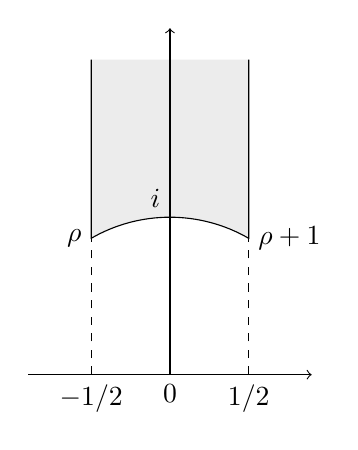
\begin{tikzpicture}[scale=2]
        \fill[gray!15] (-0.5,2) -- (-0.5,{sqrt(3)/2}) arc[start angle=120,end angle=60,radius=1] -- (0.5,2) -- cycle;
        \draw[->] (-0.9,0) -- (0.9,0);
        \draw[->] (0,0) -- (0,2.2);
        \draw (-0.5,2) -- (-0.5,{sqrt(3)/2}) arc[start angle=120,end angle=60,radius=1] -- (0.5,2);
        \draw[dashed] (-0.5,0) -- (-0.5,{sqrt(3)/2});
        \draw[dashed] (0.5,0) -- (0.5,{sqrt(3)/2});
        \node[below] at (-0.5,0) {$-1/2$};
        \node[below] at (0,0) {$0$};
        \node[below] at (0.5,0) {$1/2$};
        \node[left] at (-0.5,{sqrt(3)/2}) {$\rho$};
        \node[right] at (0.5,{sqrt(3)/2}) {$\rho + 1$};
        \node[above left] at (0,1) {$i$};
        \node at (0.25,1.65) {$\calD$};
    \end{tikzpicture}
\end{center}

\begin{proposition}\label{Prop:MF_standard_fundamental_domain}
    \leavevmode
    \begin{enumerate}
        \item The restriction $\pi : \calD \to Y$ is surjective.
        \item If $z_1, z_2 \in \calD$ are distinct and $\gamma z_1 = z_2$ for some $\gamma \in \SL_2(\bbZ)$, then either $\Re(z_1) = \pm 1/2$ and $z_2 = z_1 \mp 1$, or $|z_1| = 1$ and $z_2 = -1/z_1$.
        \item The elliptic points in $\calH$ for $\SL_2(\bbZ)$ form the two orbits $\SL_2(\bbZ)i$ and $\SL_2(\bbZ)\rho$. Their stabilizers are
        \[
            \SL_2(\bbZ)_i = \langle S\rangle, \qquad \SL_2(\bbZ)_\rho = \langle ST\rangle,
        \]
        of orders $4$ and $6$, respectively, where
        \[
            S = \begin{pmatrix}0 & -1\\ 1 & 0\end{pmatrix}, \qquad T = \begin{pmatrix}1 & 1\\ 0 & 1\end{pmatrix}, \qquad ST = \begin{pmatrix}0 & -1\\ 1 & 1\end{pmatrix}.
        \]
    \end{enumerate}
\end{proposition}

\begin{proof}
    \leavevmode
    \begin{enumerate}
        \item Fix $z \in \calH$. For every $A > 0$, the set $\{(c, d) \in \bbZ^2 \mid |cz + d| < A\}$ is finite: $|c|\Im(z) < A$ bounds $c$, and then $|c\Re(z) + d| < A$ bounds $d$. Since
        \[
            \Im(\gamma z) = \frac{\Im(z)}{|cz + d|^2},
        \]
        there exists $\gamma' \in \SL_2(\bbZ)$ for which $\Im(\gamma'z)$ is maximal. Choose $n \in \bbZ$ such that $w = T^n\gamma'z$ satisfies $|\Re(w)| \le 1/2$. Translation does not change the imaginary part, so $w$ still has maximal imaginary part. If $|w| < 1$, then
        \[
            \Im(Sw) = \frac{\Im(w)}{|w|^2} > \Im(w),
        \]
        a contradiction. Hence $w \in \calD$.
        \item We prove (2) and (3) together. Let $z \in \calD$ and $\gamma = \begin{pmatrix}a & b\\ c & d\end{pmatrix} \in \SL_2(\bbZ)$ with $\gamma z \in \calD$. Exchanging $(z, \gamma)$ with $(\gamma z, \gamma^{-1})$ if necessary, assume $\Im(\gamma z) \ge \Im(z)$. Writing $z = x + iy$, this gives
        \[
            |cz + d|^2 = (cx + d)^2 + c^2y^2 \le 1.
        \]
        Since $z \in \calD$, we have $y^2 \ge 1 - x^2 \ge 3/4$, and hence $c \in \{-1, 0, 1\}$.
        \begin{enumerate}[label=\textit{Case~\arabic*.}]
            \item $c = 0$.
            Then $a = d = \pm 1$, so $\gamma$ acts by an integral translation. Since $z$ and $\gamma z$ lie in the strip $|\Re(w)| \le 1/2$, either $\gamma = \pm\Id$, or the translation is by $\pm 1$ and exchanges the two vertical boundaries.
            \item $c = 1$.
            The inequality $|z + d| \le 1$ forces $d = 0$, except that $d = 1$ is also possible for $z = \rho$ and $d = -1$ for $z = \rho + 1$.
            % Reconstructed details: complete the boundary cases obscured in the photographs.
            If $d = 0$, then $b = -1$ and $\gamma z = a - 1/z$. The conditions $|z| \ge 1$ and $|z| \le 1$ give $|z| = 1$, so $-1/z = -\overline z$. Thus $a = 0$ except at the endpoints: for $z = \rho$, $a = 0, -1$, and for $z = \rho + 1$, $a = 0, 1$. These give either the circular boundary identification or a fixed endpoint.

            If $z = \rho$ and $d = 1$, then $a - b = 1$ and
            \[
                \gamma\rho = a - \frac{1}{\rho + 1} = a + \rho.
            \]
            Hence $a = 0, 1$. Similarly, for $z = \rho + 1$ and $d = -1$, we obtain $\gamma z = a + z$ with $a = 0, -1$. These again give a fixed endpoint or the identification of the two endpoints.
            \item $c = -1$.
            Replace $\gamma$ by $-\gamma$, which has the same action on $\calH$, and apply the preceding case.
        \end{enumerate}
        This proves (2). The same classification with $\gamma z = z$ shows that, inside $\calD$, a noncentral stabilizer is possible only at $i$, $\rho$, or $\rho + 1$. At $i$, the matrices are $\{\pm\Id, \pm S\} = \langle S\rangle$. At $\rho$, they are $\{\pm\Id, \pm ST, \pm(ST)^2\} = \langle ST\rangle$. The point $\rho + 1$ is equivalent to $\rho$ by $T$, so its stabilizer is conjugate to that of $\rho$. Part (1) now gives (3) for all of $\calH$.
    \end{enumerate}
\end{proof}

\begin{remark}
    Parts (1) and (2) say that $\calD$ is a fundamental domain for the action of $\SL_2(\bbZ)$ on $\calH$.
\end{remark}

\begin{corollary}\label{Cor:MF_finite_elliptic_points}
    Let $\Gamma$ be a congruence subgroup. Then $Y(\Gamma)$ has finitely many elliptic points, and every elliptic stabilizer $\Gamma_z$ is finite cyclic.
\end{corollary}

\begin{proof}
    For every $z \in \calH$, we have $\Gamma_z \subseteq \SL_2(\bbZ)_z$. By \propref{Prop:MF_standard_fundamental_domain}, the latter is finite cyclic, and hence so is $\Gamma_z$. This also proves \propref{Prop:MF_elliptic_stabilizer}.

    Write $\SL_2(\bbZ) = \bigcup_{j=1}^r\Gamma\delta_j$, where $r = [\SL_2(\bbZ) : \Gamma] < \infty$. Every point elliptic for $\Gamma$ is elliptic for $\SL_2(\bbZ)$, so its $\Gamma$-orbit is among
    \[
        \{\Gamma\delta_j i,\ \Gamma\delta_j\rho \mid 1 \le j \le r\}.
    \]
    There are at most $2r$ such orbits.
\end{proof}

\subsection{The Compact Modular Curves}\label{Sec:MF_compact_modular_curves}

Let $\calH^* := \calH \cup \bbQ \cup \{\infty\}$. Recall that $\SL_2(\bbZ)$ acts transitively on $\bbQ \cup \{\infty\}$, and
\[
    \SL_2(\bbZ)_\infty = \left\{\pm\begin{pmatrix}1 & n\\ 0 & 1\end{pmatrix} \ \middle|\ n \in \bbZ\right\}.
\]

\begin{definition}[Compact Modular Curve]\label{Def:MF_compact_modular_curve}
    The \termino{compact modular curve} associated with a congruence subgroup $\Gamma$ is
    \[
        X(\Gamma) := \Gamma \backslash \calH^* = Y(\Gamma) \cup \bigl(\Gamma \backslash (\bbQ \cup \{\infty\})\bigr).
    \]
    Thus $X(\Gamma)$ is obtained from $Y(\Gamma)$ by adding the finitely many cusps of $\Gamma$. For $N \in \bbN_{>0}$, write
    % Source notation: the board writes X_1(Gamma_1(N)) on the left of the middle definition, apparently in place of X_1(N).
    \[
        X(N) := X(\Gamma(N)), \qquad X_1(N) := X(\Gamma_1(N)), \qquad X_0(N) := X(\Gamma_0(N)).
    \]
\end{definition}

For $M \in \bbR_{>0}$, put
\[
    \mathcal{N}_M := \{z \in \calH \mid \Im(z) > M\}.
\]
Equip $\calH^*$ with the topology generated by the open subsets of $\calH$ and the sets
\[
    \alpha\bigl(\mathcal{N}_M \cup \{\infty\}\bigr), \qquad \alpha \in \SL_2(\bbZ),\ M > 0.
\]
Every $\gamma \in \SL_2(\bbZ)$ acts on $\calH^*$ by a homeomorphism. We equip $X(\Gamma)$ with the quotient topology for the natural projection $\pi^* : \calH^* \to X(\Gamma)$.

\begin{remarkstar}
    In the next lecture, we will prove that $X(\Gamma)$ is Hausdorff, connected and compact.
\end{remarkstar}
